\subsection*{Zadatak Kraljevstvo}
\textsf{Pripremili: Tonko Sabolčec i Paula Vidas}\\
\textsf{Potrebno znanje: geometrija, konveksna ljuska, dinamičko programiranje, metoda \textit{podijeli pa vladaj}}

Za prvi podzadatak dovoljno je za svaki $K$-člani podskup dvoraca koji sadrži
najljeviji i najdesniji dvorac izračunati površinu konveksne ljuske pripadajućih
točaka iz podskupa. Za određivanje konveksne ljuske određenog skupa točaka
preporučuje se korištenje \textit{monotone chain} algoritma, dok se površina
konveksnog poligona može dobiti podjelom poligona na $K - 2$ trokuta (npr.
koji dijele jedan zajednički vrh) i zbrajanjem površina trokuta dobivenih preko
analitičke formule:
\begin{equation*}
  P(\Delta ABC) = \frac{1}{2} \cdot |x_A(y_B - y_C) + x_B(y_C - y_A) + x_C(y_A - y_B)|.
\end{equation*}

Ostalim podzadacima pristupit ćemo tako da zadani skup točaka podijelimo na one
iznad i ispod $x$-osi (pri čemu najljeviju i najdesniju točku uzimamo u oba
skupa) te odredimo optimalne donje i gornje polovice konačne ljuske. Konkretnije,
izračunat ćemo vrijednosti $up(k)$ i $down(k)$ za svaki $2 \le k \le K$ gdje
$up(k)$ predstavlja najveću moguću površinu neke ljuske koja se sastoji od $k$
vrhova gornjeg skupa točaka, dok $down(k)$ predstavlja analogne vrijednosti za
donji skup točaka. Također primijetite da nas zanimaju ljuske koje se sastoje
od $K$ ili \textit{manje} vrhova. Konačno rješenje tada dobivamo pronalaskom najvećeg zbroja
$up(k_1) + down(k_2)$ pri čemu je $k_1 + k_2 \le K + 2$ (ova dvojka proizlazi iz
činjenice što smo najljeviju i najdesniju točku koristili u oba skupa).

Vrijednosti $up(k)$ i $down(k)$ možemo dobiti primjenom dinamičkog programiranja.
U nastavku ćemo se usredotočiti samo na gornju polovicu točaka (obrada za donju
polovicu ide analogno). Neka su $P_1, P_2, ..., P_n$ točke gornje polovice
uzlazno sortirane po $x$-koordinati ($P_1$ je najljevija, a $P_n$ najdesnija).
Označimo s $dp(k,i,j)$ najveću moguću površinu neke konveksne ljuske prvih
$j$ točaka ($P_1, P_2, ..., P_j$) koja se sastoji od $k$ vrhova, pri čemu su
$P_i$ i $P_j$ posljednja dva vrha. Stanje gradimo prijelazima u kojima dodajemo
po jednu sljedeću točku gornje ljuske uz pribrajanje pripadajuće površine.
U stanje $dp(k,i,j)$ mogli smo doći iz stanja $dp(k-1,i',i)$ uz pribrajanje
površine trokuta $P(\Delta P_1P_iP_j)$, koju ćemo označiti s $w(i, j)$.
Pritom je važno voditi računa o
konveksnosti vrhova koje uzimamo, tj. da točke $P_i', P_i, P_j$ budu poredane
u smjeru kazaljke na satu.

\begin{figure}[h]
  \centering
  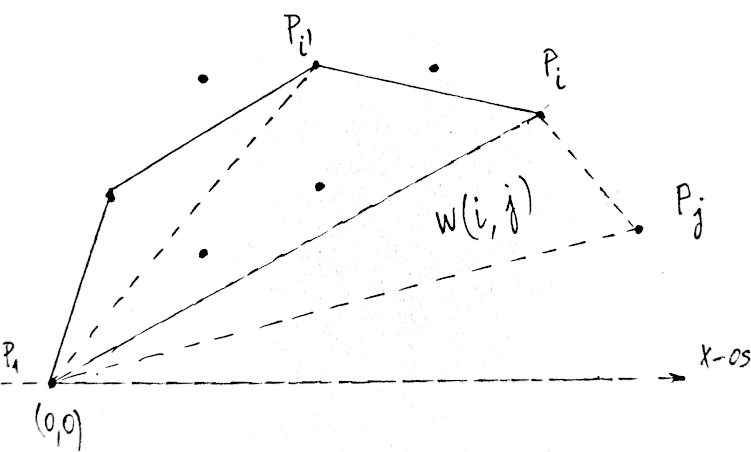
\includegraphics[height=4.5cm]{pic/img1.png}
\end{figure}

Možemo pisati:
\begin{equation*}
  dp(k,i,j) = \text{max}_{1 \le i' < i} \{ dp(k-1,i',i) + w(i, j)\}
  \ \text{ t.d. }\
  ccw(P_i', P_i, P_j) < 0,
\end{equation*}
pri čemu je $ccw(A, B, C)$ negativna ako su točke $A, B, C$ poredane u smjeru
kazaljke na satu. Konkretna vrijednost $ccw$ funkcije može se dobiti vektorskim
množenjem vektora $\overrightarrow{AB}$ i $\overrightarrow{AC}$:
\begin{equation*}
  ccw(A, B, C) = \overrightarrow{AB} \times \overrightarrow{AC} =
    (x_B - x_A)(y_C - y_A) - (x_C - x_A)(y_B - y_A).
\end{equation*}
Vrijednosti početnih stanja $dp(2,1,i)$ jednake su nuli, a konačna vrijednost
$up(k)$ dobiva se kao $up(k) = \max_{1 < i < n} dp(k,i,n)$. Stanja ima
$\mathcal{O}(K \cdot N^2)$, a složenost prijelaza je $\mathcal{O}(N)$ pa
je ukupna složenost takvog algoritma $\mathcal{O}(K \cdot N^3)$, dovoljna
za osvajanje bodova na drugom podzadatku.

\newtheorem{zamjedba}{Zamjedba}

\begin{zamjedba}
Vrhovi optimalne konveksne ljuske bit će podskup vrhova konveksne ljuske svih ulaznih
točaka.
\end{zamjedba}

\begin{proof}[Skica dokaza]
  Neka je $H$ skup vrhova konveksne ljuske svih ulaznih točaka (točke
  tog skupa nazvat ćemo \textit{vanjskim} točkama). Pretpostavimo suprotno, tj.
  da je za određenu veličinu ljuske, optimalna konveksna ljuska $H' \not\subset H$. Drugim riječima $H'$ sadrži
  točku koja nije \textit{vanjska}, neka je to točka $H'_i$. (Na slici ispod vanjske
  su točke popunjene.) Provucimo pravac kroz vrhove susjedne vrhu
  $H'_i$ odabrane konveksne ljuske, tj. kroz točke $H'_{i-1}$ i $H'_{i+1}$.
  Tražimo najudaljeniju točku (nazovimo je $X$) od promatranog pravca s iste strane
  pravca kao točka $H'_i$. Najudaljenija točka $X$ sigurno je različita od $H'_i$ te
  pripada vanjskoj ljusci $H$ (kad bi $H'_i$ bila najudaljenija točka, tada bi $H'_i$
  ujedno bila i dio vanjske ljuske, što je suprotno pretpostavci). Primjetite da
  se zamjenom točke $H'$ točkom $X$ povećava površina odabrane konveksne ljuske
  (što proizlazi iz formule za trokut $\frac{1}{2} \cdot baza \cdot visina$).
  No, to je u kontradikciji s pretpostavkom da je polazna konveksna ljuska bila
  optimalne površine.
\end{proof}

\begin{figure}[h]
  \centering
  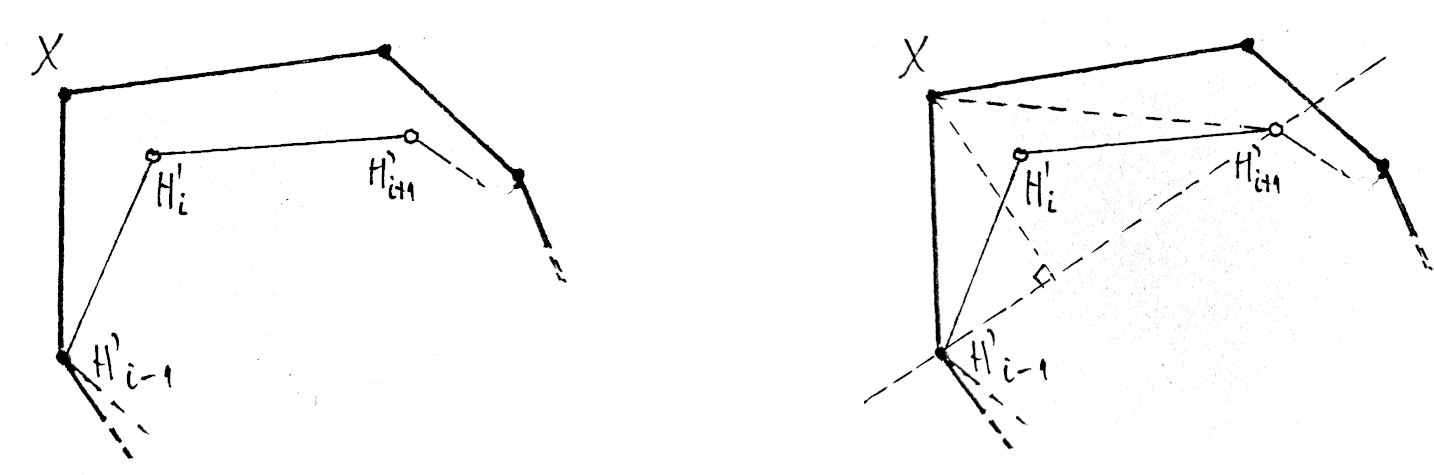
\includegraphics[height=4cm]{pic/img2.png}
\end{figure}

Razlog zbog kojeg smo u prethodno opisanoj dinamici pamtili posljednje dvije
točke u stanju je taj da omogućimo postupnu izgradnju konveksne ljuske na \textit{proizvoljnom}
skupu točaka (treću točku u prijelazu uvijek smo birali tako da se zadovolji smjer kazaljke
na satu). No, sada možemo zanemariti sve točke koje nisu vrhovi konveksne
ljuske ulaznih točaka, umjesto zadnje dvije točke u stanju možemo pamtiti
samo posljenju točku. Drugim riječima, stanje dinamike $dp(k,i)$ predstavlja
najveću moguću površinu neke konveksne ljuske koja se sastoji od $k$ vrhova
pri čemu je posljednji vrh točka $P_i$. Prijelaz se tada može zapisati kao:
\begin{equation*}
  dp(k,i) = \text{max}_{1 \le j < i}\ \{ dp(k-1, j) + w(j, i) \}.
\end{equation*}
Pritom se pretpostavlja da točke $P_1, P_2, ... P_n$ čine vrhove gornje
konveksne ljuske.
Postoji $\mathcal{O}(K \cdot N)$ stanja, a složenost prijelaza je $\mathcal{O}(N)$, što
daje ukupnu vremensku složenost od $\mathcal{O}(K \cdot N^2)$, što je dovoljno za
treći podzadatak.

\begin{zamjedba}
  \label{quadrangle}
  Za oznake pozicija $a < b < c < d$ vrijedi $w(a,d) + w(b,c) < w(a,c) + w(b,d)$.
\end{zamjedba}

\begin{proof}[Skica dokaza]
  Spomenuta nejednakost popularno se naziva \textit{nejednakost četverokuta}, a u našem će
  slučaju poslužiti kao trik za optimizaciju dinamike. No, obrazložimo
  za početak tu tvrdnju. Vrijednost $w(i,j)$ jednaka je:
  \begin{equation*}
    w(i,j) = P(\Delta P_1P_iP_j) = P((0, 0), P_i, P_j) = \frac{1}{2}(x_j y_i - x_i y_j),
  \end{equation*}
  gdje je $P_i = (x_i, y_i)$. Raspisivanjem, preslagivanjem i sređivanjem
  dobiva se:
  \begin{equation*}
    w(a,d) + w(b,c) - w(a,c) - w(b,d) = \frac{1}{2}((x_b - x_a)(y_d - y_c) - (y_b - y_a)(x_d - x_c)).
  \end{equation*}
  Izraz s desne strane odgovara polovici vektorskog umnoška $\overrightarrow{P_a P_b} \times
  \overrightarrow{P_c P_d}$, a budući da su točke $P_a, P_b, P_c, P_d$ poredane u
  smjeru kazaljke na satu, ta je vrijednost negativna, tj. vrijedi:
  \begin{equation*}
    w(a,d) + w(b,c) - w(a,c) - w(b,d) < 0\ \ \Rightarrow\ \
    w(a,d) + w(b,c) < w(a,c) + w(b,d).
  \end{equation*}
\end{proof}

\begin{zamjedba}
  Neka je $p_{k,i}$ oznaka najmanje vrijednosti $j$ optimalnog prijelaza u
  $dp(k,i) = dp(k-1,j) + w(j, i)$. Tada vrijedi $p_{k,i+1} \ge p_{k,i}$.
\end{zamjedba}

\begin{proof}[Skica dokaza]
  Pretpostavimo suprotno, tj. da za neke $k, i$
  vrijedi $p_{k,i+1} < p_{k,i}$. Budući da je $p_{k,i}$ optimalni prijelaz
  za $dp(k,i)$, odnosno $p_{k,i+1}$ optimalni prijelaz za $dp(k,i+1)$,
  vrijede nejednakosti:
  \begin{equation*}
    \begin{aligned}
      dp(k-1,p_{k,i}) + w(p_{k,i}, i) &\geq dp(k-1,p_{k,i+1}) + w(p_{k,i+1},i) \\
      dp(k-1,p_{k,i+1}) + w(p_{k,i+1},i+1) &\geq dp(k-1,p_{k,i}) + w(p_{k,i},i+1)
    \end{aligned}
  \end{equation*}
  Zbrajanjem nejednakosti i sređivanjem dolazi se do:
  \begin{equation*}
    w(p_{k,i},i) + w(p_{k,i+1},i+1) \geq w(p_{k,i+1},i) + w(p_{k,i},i+1).
  \end{equation*}
  Po pretpostavci vrijedi $p(k,i+1) < p(k,i) < i < i+1$, pa primjenom
  \textit{Zamjedbe \ref{quadrangle}} dobivamo:
  \begin{equation*}
    w(p_{k,i},i) + w(p_{k,i+1},i+1) < w(p_{k,i+1},i) + w(p_{k,i},i+1).
  \end{equation*}
  što je u kontradikciji s prije dobivenom nejednakosti. Zaključujemo
  da vrijedi $p(k,i+1) \geq p(k,i)$.
\end{proof}
 
Konačno ćemo dobivene spoznaje iskoristiti za optimiziranje naše dinamike!
Pretpostavimo da smo odredili sve vrijednosti $dp(k-1,i)$ i da na temelju
njih želimo izračunati vrijednosti $dp(k,i)$ za svaki $1 \le i \le n$.
Najprije ćemo izračunati $dp(k,n/2)$, tako da prođemo po svim $1 \le j < n/2$
i odredimo optimalni prijelaz $p_{k,n/2}$. Zbog $p_{k,i+1} \ge p_{k,i}$ optimalni prijelaz
za $dp_{k,i<n/2}$ dobiva se u intervalu $p_{k,i<n/2} \in [1, p_{i,n/2}]$,
dok je za $i>n/2$ ta vrijednost u intervalu $p_{k,i>n/2} \in [p_{i,n/2},n]$.
Izračun svih vrijednosti $dp(k,i)$ stoga se može obaviti rekurzivnom metodom
\textit{podijeli pa vladaj} u kojoj pamtimo dva intervala. Prvi interval,
$[lo, hi]$, odnosi se na vrijednosti $i$ za koje želimo izračunati $dp(k, i)$,
a drugi interval $[p_{lo}, p_{hi}]$ odnosi se na granice u kojima se traži
optimalni prijelaz $p_{k,i}$. Pseudokod rekurzivne funkcije dan je u nastavku:
\begin{verbatim}
izracunaj(lo, hi, p_lo, p_hi):
    mid = (lo + hi) / 2
    p_opt = 0
    dp(k, i) = 0
    za svaki i := p_lo do min(mid-1, p_hi):
        ako dp(k-1, i) + w(i, mid) > dp(k, i):
            dp(k, i) = dp(k-1, i) + w(i, mid)
            p_opt = i
    izracunaj(lo, mid-1, p_lo, p_opt)
    izracunaj(mid+1, hi, p_opt, p_hi)
\end{verbatim}

Rekurziju je potrebno pozvati s parametrima $izracunaj(1, n, 1, n)$, a može se
pokazati da je složenost takvog poziva $\mathcal{O}(N \log N)$. Budući da funkciju
moramo pozvati $K$ puta (za svaki prijelaz s $k-1$ na $k$), ukupna složenost
algoritma iznosi $\mathcal{O}(K \cdot N \log N)$.

\textbf{Alternativno rješenje:} Umjesto da maksimiziramo površinu konveksne
ljuske odabranih točaka, ekvivalentno je minimizirati razliku površina konveksne
ljuske svih točaka i odabranih točaka. Stanje dinamike $dp(k, i)$ je tada
najmanja moguća razlika površina konveksne ljuske točaka $P_1, P_2, \dots, P_i$
i konveksne ljuske nekog $k$-članog podskupa tih točaka koji sadrži $P_1$ i
$P_i$. Naivna implementacija te dinamike ima složenost $\mathcal{O}(K \cdot
N^2)$, a može se ubrzati koristeći tzv. \textit{Knuthovu optimizaciju} do
složenosti $\mathcal{O}(N^2)$. Detaljnu analizu ovog pristupa ostavljamo
čitatelju za vježbu, a više o Knuthovoj optimizaciji možete pročitati
\href{https://jeffreyxiao.me/blog/knuths-optimization}{ovdje} i
\href{https://wiki.algo.is/Knuth's\%20optimization}{ovdje}.
